
%(BEGIN_QUESTION)
% Copyright 2007, Tony R. Kuphaldt, released under the Creative Commons Attribution License (v 1.0)
% This means you may do almost anything with this work of mine, so long as you give me proper credit

Graph the response of a proportional+integral controller with a proportional band of 50\% and an integral constant of 1.25 minutes per repeat to the following input conditions.  Assume a control action that is {\it reverse-acting}:

$$\includegraphics[width=15.5cm]{i01604x01.eps}$$

The time scale on the chart is minutes:seconds, and the PI algorithm is as follows:

$$m = K_p \left( e + {1 \over \tau_i} \int e \> dt \right) + b$$

\noindent
Where,

$m$ = Controller output (manipulated variable)

$K_p$ = Gain

$e$ = Error signal (SP$-$PV)

$\tau_i$ = Integral time constant

$b$ = Bias

\vskip 10pt

\underbar{file i01604}
%(END_QUESTION)





%(BEGIN_ANSWER)

$$\includegraphics[width=15.5cm]{i01604x02.eps}$$

To the PV step-change of -10\%, the controller immediately responds with an output step-change of 20\% (the proportional band value of 50\% is the same as a gain of 2), bringing the output from its original value of 20\% to 40\%.  Then, the continuing error of -10\% causes the integral action to ramp the output signal at a rate of 16\% per minute (20\% proportional response multiplied by 0.8 repeats per minute).  Since the -10\% deviation between PV and SP only lasts 30 seconds (between 0:15 and 0:45), the output signal only gets the chance to ramp up 8\%, bringing the output to a value of 48\% at the end of the first deviation period.

Then, when the PV returns to SP (a +10\% step-change), the output jumps downward by 20\%, leaving the output 8\% higher than where it began (28\%, from the original value of 20\%).

When the next PV step-change arrives at 1:30, the +5\% step upwards causes an immediate -10\% step in output due to proportional action, bringing the output value to 18\%.  Integral action, working at a rate of 0.8 repeats per minute, takes the proportional response of -10\% and produces an output slope of -8\% per minute.  Since this step-change period lasts only 10 seconds (1:30 to 1:40), the accumulated output change due to integral is -1.333\%, bringing the output down to a final low value of 16.67\%.  When the PV returns back to SP (jumping down 5\%), the output jumps up by 10\%, leaving the final output value at 26.67\% until the end of the graph.

%(END_ANSWER)





%(BEGIN_NOTES)


%INDEX% Control, proportional + integral: graphing controller response

%(END_NOTES)


